\documentclass[11pt,letterpaper]{article}

\usepackage[margin=1in,headheight=14pt]{geometry}
\usepackage{amsmath,amssymb,amsthm,mathtools}
\usepackage{graphicx}
\usepackage{xcolor}
\usepackage{enumitem}
\usepackage{microtype}
\usepackage{fancyhdr}
\usepackage[colorlinks=true,linkcolor=blue,citecolor=blue,urlcolor=blue]{hyperref}

% Personal notation and theorem environments.
%!TEX root = EM_singular_models.tex

% PDF margin etc settings
%\setlength{\textwidth}{\paperwidth}
%\addtolength{\textwidth}{-6cm}
%\setlength{\textheight}{\paperheight}
%\addtolength{\textheight}{-4cm}
%\addtolength{\textheight}{-1.1\headheight}
%\addtolength{\textheight}{-\headsep}
%\addtolength{\textheight}{-\footskip}
%\setlength{\oddsidemargin}{0.5cm}
%\setlength{\evensidemargin}{0.5cm}

%%%%%%%%%%%%%%%%%%%%%%%%%%%%%%%%

% MACROS HERE

%%%%%%%%%%%%%%%%%%%%%%%%%%%%%%%%

\newcommand{\fixedpointtheta}{\widehat\theta_\obs}

\newcommand{\cover}{N}
\newcommand{\kinit}{\nu}
\newcommand{\cdelta}{c_\threshold}
\newcommand{\dndelta}{\omega}
\newcommand{\kndelta}{\Upsilon}
\newcommand{\kndeltanew}{\Psi}
\newcommand{\radii}{\mathcal{R}}
\newcommand{\event}{\mathcal{E}}
\newcommand{\kevent}{\mathcal{D}}


% Observations, dimension etc.
\newcommand{\dims}{\ensuremath{d}}
\newcommand{\samples}{\ensuremath{n}}
\newcommand{\obs}{\samples}
\newcommand{\real}{\ensuremath{\mathbb{R}}}
\newcommand{\complex}{\ensuremath{\mathbb{C}}}
\newcommand{\realdim}{\ensuremath{\real^\dims}}

\newcommand{\smallthreshold}{\epsilon}

% some mathcal notations
\newcommand{\order}[1]{\ensuremath{\mathcal{O}\parenth{#1}}}

% Basic statistics notation
\newcommand{\xstar}{\ensuremath{x^*}}
\newcommand{\xbar}{\ensuremath{\bar{x}}}
% True parameter
\newcommand{\thetastar}{\ensuremath{{\theta^*}}}
% Estimate one
\newcommand{\thetahat}{\ensuremath{\widehat{\theta}}}
% Estimate two
\newcommand{\thetatil}{\ensuremath{\widetilde{\theta}}}
\newcommand{\thetabar}{\ensuremath{\bar{\theta}}}
\newcommand{\yvec}{\ensuremath{y}}
\newcommand{\Xmat}{\ensuremath{X}}

% Distributions
\newcommand{\distribution}{P}
\newcommand{\density}{f}
\newcommand{\gaussiandensity}{\phi}
\newcommand{\NORMAL}{\ensuremath{\mathcal{N}}}
\newcommand{\BER}{\ensuremath{\mbox{Ber}}}

% Spaces
\newcommand{\Xspace}{\ensuremath{\mathcal{X}}}
\newcommand{\Yspace}{\ensuremath{\mathcal{Y}}}
\newcommand{\Zspace}{\ensuremath{\mathcal{Z}}}


% Brackets Size
\newcommand{\brackets}[1]{\left[ #1 \right]}
\newcommand{\parenth}[1]{\left( #1 \right)}
\newcommand{\bigparenth}[1]{\big( #1 \big)}
\newcommand{\biggparenth}[1]{\bigg( #1 \bigg)}
\newcommand{\braces}[1]{\left\{ #1 \right \}}
\newcommand{\abss}[1]{\left| #1 \right |}
\newcommand{\angles}[1]{\left\langle #1 \right \rangle}
\newcommand{\tp}{^\top}

% Generic vectors and scalars
\newcommand{\myvec}{u} % for generic vector
\newcommand{\myvectwo}{v} % for generic vector
\newcommand{\mymat}{B}
\newcommand{\set}{{A}}
\newcommand{\scalar}{\alpha}
\newcommand{\tvscalar}{\epsilon}
\newcommand{\tailboundscalar}{t}
\newcommand{\term}{U}
\newcommand{\myVarone}{\alpha_X}
\newcommand{\myVartwo}{\alpha_Y}
\newcommand{\myCovmat}{\Sigma}
\newcommand{\xcord}[1]{x^{(#1)}}
\newcommand{\xcordpop}[1]{X^{(#1)}}
\newcommand{\ycordpop}[1]{Y^{(#1)}}
\newcommand{\myVarthree}{\ensuremath{U}}
\newcommand{\myVarfour}{\ensuremath{V}}
\newcommand{\myfuntwo}{\ensuremath{g}}
\newcommand{\numsteps}{t}
\newcommand{\totalnumsteps}{T}
\newcommand{\seqalpha}[1]{\alpha_{#1}}
\newcommand{\seqnu}[1]{\nu^{(#1)}}
\newcommand{\imax}{\ell_\smallthreshold}
\newcommand{\basis}{e}
\newcommand{\radem}{\varepsilon}
\newcommand{\Tone}{T\ensuremath{_{0}}}
\newcommand{\Ttwo}{T\ensuremath{_{2}}}
\newcommand{\contractPar}[1]{\ensuremath{\gamma\parenth{#1}}}

\newcommand{\simiid}{\overset{\mathrm{i.i.d.}}{\sim}}
\newcommand{\eqd}{\overset{d}{=}}


% EM updates
\newcommand{\hidden}{Z}
\newcommand{\qfun}[2]{Q(#1\vert#2)}
\newcommand{\variable}{\theta}
\newcommand{\weights}{w}
\newcommand{\myfun}{q}
\newcommand{\gradf}{\nabla \myfun}
\newcommand{\hessf}{\nabla^2 \myfun}
\newcommand{\iter}{t}
\newcommand{\mupdate}{M}
\newcommand{\mupdategeneral}{\ensuremath{M^{GN}}}




% EM contractions
\newcommand{\contractgene}{\ensuremath{\gamma^{GN}}}
\newcommand{\updateMat}{\ensuremath{\Gamma_{\theta}}}
\newcommand{\mymatTheta}{\ensuremath{B_{\theta}}}
\newcommand{\sech}{\text{sech}}

% Nhat's macros 
\newcommand{\Rspace}{\ensuremath{\mathbb{R}}}
\newcommand{\Ecal}{\ensuremath{\mathcal{E}}}
\newcommand{\Ncal}{\ensuremath{\mathcal{N}}}
\newcommand{\gradient}{\ensuremath{\nabla}}
\newcommand{\smallweight}{\ensuremath{\epsilon^{sw}}}
\newcommand{\smallnorm}{\ensuremath{\rho^{sw}}}
\newcommand{\ball}{\ensuremath{\mathbb{B}}}
\newcommand{\sphere}{\ensuremath{\mathbb{S}}}

\newcommand{\diam}{\ensuremath{\text{diam}}}
\newcommand{\upper}{\ensuremath{\bar{C}}}
\newcommand{\sample}{\ensuremath{\xi}}
\newcommand{\weight}{\ensuremath{\pi}}
\newcommand{\contracasym}{\ensuremath{\rho}}
\newcommand{\Fishermatrix}{\ensuremath{\mathcal{I}}}
\newcommand{\barcontracasym}{\ensuremath{\bar{\rho}}}


\newcommand{\TrueDensity}{\ensuremath{f}}
\newcommand{\FitDensity}{\ensuremath{f}_{\theta}}
\newcommand{\FitDensityfree}{\ensuremath{f}_{\pi, \theta}}
\newcommand{\FitDensitygen}{\ensuremath{f}_{\pi, \theta_{1}, \theta_{2}}}
\newcommand{\FitDensitymore}{\ensuremath{f}_{G}}
\newcommand{\normden}{\ensuremath{\phi}}
\newcommand{\mean}{\ensuremath{\theta}}
\newcommand{\sd}{\ensuremath{\sigma}}
\newcommand{\parFOS}{\ensuremath{\gamma}}
\newcommand{\funQ}{\ensuremath{Q}}
\newcommand{\updateM}{\ensuremath{M}}
\newcommand{\weightFun}{\ensuremath{w}}
\newcommand{\mydefn}{\ensuremath{:=}}
\newcommand{\poincare}{\ensuremath{\tilde{C}}}
\newcommand{\paraspace}{\ensuremath{\Theta}}
\newcommand{\loglihood}{\ensuremath{F}}
\newcommand{\prior}{\ensuremath{\pi}}
\newcommand{\posterior}{\ensuremath{\Pi}}
\newcommand{\boundcons}{\ensuremath{B}}
\newcommand{\boundconstot}{\ensuremath{H}}
\newcommand{\noise}{\ensuremath{\varepsilon}}
\newcommand{\loglihoodgaus}{\ensuremath{F^{G}}}
\newcommand{\loglihoodind}{\ensuremath{F^{I}}}
\newcommand{\loglihoodlogit}{\ensuremath{F^{R}}}
\newcommand{\noiseone}{\ensuremath{\varepsilon_{1}}}
\newcommand{\noisetwo}{\ensuremath{\varepsilon_{2}}}

%%%SDE_Bayesian_inf
\newcommand{\weakcon}{\ensuremath{\psi}}
\newcommand{\perturb}{\ensuremath{\zeta}}
\newcommand{\inver}{\ensuremath{\xi}}

% Universal constants
\newcommand{\unicon}{c}
\newcommand{\uniconnew}{c'}
\newcommand{\uniconone}{c_1}
\newcommand{\unicontwo}{c_2}

% some parameters that you may define
\newcommand{\scparam}{m} % strong  convexity parameter
\newcommand{\smoothness}{L} % smoothness parameter
\newcommand{\step}{h}


%%%%%%%%% Distributions and Random variables %%%%%%%%%%%
\newcommand{\rvg}{\xi} % to denote the random variable g
\newcommand{\threshold}{\delta}


%%%%%%%%% Basic Terms like defn, etal, tmix, polylog %%%%%%%%%%%
\newcommand{\defn}{:=}
\newcommand{\rdefn}{=:}
\newcommand{\etal}{{et al.}}
\newcommand{\polylog}{\text{poly-log}}

% Some vector/matrix norms
\newcommand{\matnorm}[3]{|\!|\!| #1 | \! | \!|_{{#2}, {#3}}}
\newcommand{\matsnorm}[2]{|\!|\!| #1 | \! | \!|_{{#2}}}
\newcommand{\vecnorm}[2]{\left\| #1\right\|_{#2}}
\newcommand{\enorm}[1]{\vecnorm{#1}{2}} % euclidean norm
\newcommand{\nucnorm}[1]{\ensuremath{\matsnorm{#1}{\footnotesize{\mbox{nuc}}}}}
\newcommand{\fronorm}[1]{\ensuremath{\matsnorm{#1}{\footnotesize{\mbox{fro}}}}}
\newcommand{\opnorm}[1]{\ensuremath{\matsnorm{#1}{\tiny{\mbox{op}}}}}
%%% EM paper
\newcommand{\constrainnorm}[1]{\vecnorm{#1}{[k]}} % euclidean norm

\newcommand{\bigmatsnorm}[2]{{\Big|\!\Big|\!\Big| #1
  \Big|\!\Big|\!\Big|}_{#2}}

% Inner product
\newcommand{\inprod}[2]{\ensuremath{\langle #1 , \, #2 \rangle}}

% Kullback-Leibler
\newcommand{\kull}[2]{\ensuremath{D_{\text{KL}}(#1\; \| \; #2)}}

% Probability
\newcommand{\Exs}{\ensuremath{{\mathbb{E}}}}
\newcommand{\Prob}{\ensuremath{{\mathbb{P}}}}

%Eigenvector / eigenvalue related notation
\newcommand{\eig}[1]{\ensuremath{\lambda_{#1}}}
\newcommand{\eigmax}{\ensuremath{\eig{\max}}}
\newcommand{\eigmin}{\ensuremath{\eig{\min}}}

% \DeclareMathOperator{\det}{det}
\DeclareMathOperator{\modd}{mod}
\DeclareMathOperator{\diag}{diag}
\DeclareMathOperator{\var}{var}
\DeclareMathOperator{\cov}{cov}
\DeclareMathOperator{\trace}{trace}
\DeclareMathOperator{\abs}{abs}
\DeclareMathOperator{\floor}{floor}
\DeclareMathOperator{\vol}{vol}
\DeclareMathOperator{\child}{child}
\DeclareMathOperator{\parent}{parent}
\DeclareMathOperator{\sign}{sign}
\DeclareMathOperator{\rank}{rank}
\DeclareMathOperator{\toeplitz}{toeplitz}




\newtheoremstyle{named}{}{}{\itshape}{}{\bfseries}{.}{.5em}{\thmnote{#3's }#1}
\theoremstyle{named}
\newtheorem*{namedtheorem}{Lemma}

%%%%%%%
\theoremstyle{plain}

% {Theorem, Proposition, Lemma, Corollary} numbered sequentially
% throughout the paper
\newtheorem{theorem}{Theorem}
\newtheorem{proposition}{Proposition}
\newtheorem{lemma}{Lemma}
\newtheorem{claim}{Claim}
\newtheorem{corollary}{Corollary}
\newtheorem{definition}{Definition}
\newtheorem{conjecture}{Conjecture}
\newtheorem{remark}{Remark}
%%%%%%%%%%%%%%%%%%%%%%%%%%%%%%%%%%%%%%%%%%%%%%%%%%%%%%%%%%%%%%%%%%%%%%%
% WIDEBAR COMMAND
\newlength{\widebarargwidth}
\newlength{\widebarargheight}
\newlength{\widebarargdepth}
\DeclareRobustCommand{\widebar}[1]{%
  \settowidth{\widebarargwidth}{\ensuremath{#1}}%
  \settoheight{\widebarargheight}{\ensuremath{#1}}%
  \settodepth{\widebarargdepth}{\ensuremath{#1}}%
  \addtolength{\widebarargwidth}{-0.3\widebarargheight}%
  \addtolength{\widebarargwidth}{-0.3\widebarargdepth}%
  \makebox[0pt][l]{\hspace{0.3\widebarargheight}%
    \hspace{0.3\widebarargdepth}%
    \addtolength{\widebarargheight}{0.3ex}%
    \rule[\widebarargheight]{0.95\widebarargwidth}{0.1ex}}%
  {#1}}



%%% New version of \caption puts things in smaller type, single-spaced
%%% and indents them to set them off more from the text.
\makeatletter
\long\def\@makecaption#1#2{
        \vskip 0.8ex
        \setbox\@tempboxa\hbox{\small {\bf #1:} #2}
        \parindent 1.5em  %% How can we use the global value of this???
        \dimen0=\hsize
        \advance\dimen0 by -3em
        \ifdim \wd\@tempboxa >\dimen0
                \hbox to \hsize{
                        \parindent 0em
                        \hfil
                        \parbox{\dimen0}{\def\baselinestretch{0.96}\small
                                {\bf #1.} #2
                                %%\unhbox\@tempboxa
                                }
                        \hfil}
        \else \hbox to \hsize{\hfil \box\@tempboxa \hfil}
        \fi
        }
\makeatother



%% COMMENTING commands

\long\def\comment#1{}
\definecolor{battleshipgrey}{rgb}{0.52, 0.52, 0.51}
\definecolor{darkgray}{rgb}{0.66, 0.66, 0.66}
\definecolor{darkgreen}{rgb}{0.0, 0.2, 0.13}
\definecolor{darkspringgreen}{rgb}{0.09, 0.45, 0.27}
\definecolor{dukeblue}{rgb}{0.0, 0.0, 0.61}
\definecolor{olivedrab7}{rgb}{0.24, 0.2, 0.12}
\definecolor{darkblue}{rgb}{0.0, 0.0, 0.55}
\definecolor{darkscarlet}{rgb}{0.34, 0.01, 0.1}
\definecolor{candyapplered}{rgb}{1.0, 0.03, 0.0}
\definecolor{ao(english)}{rgb}{0.0, 0.5, 0.0}
\definecolor{applegreen}{rgb}{0.55, 0.71, 0.0}

\newcommand{\red}[1]{\textcolor{red}{#1}}
\newcommand{\mjwcomment}[1]{{\bf{{\red{{MJW --- #1}}}}}}
\newcommand{\mwlcomment}[1]{{\bf{{\color{orange}{{Wenlong --- #1}}}}}}

\newcommand{\blue}[1]{\textcolor{blue}{#1}}
\newcommand{\green}[1]{\textcolor{green}{#1}}
\newcommand{\highlight}[1]{\textcolor{applegreen}{#1}}

% comment lines
\newcommand{\genecomment}[1]{{\bf{{\blue{{TEAM --- #1}}}}}}
\newcommand{\rrdcomment}[1]{{\bf{{\blue{{RRD --- #1}}}}}}
\newcommand{\nhcomment}[1]{{\bf{{\blue{{NH --- #1}}}}}}
\newcommand{\kkcomment}[1]{{\bf{{\darkgreen{{KK --- #1}}}}}}


\newcommand{\widgraph}[2]{\includegraphics[keepaspectratio,width=#1]{#2}}


\newcommand{\coursenumber}{STA3000F}
\newcommand{\coursetitle}{Advanced Theory of Statistics}
\newcommand{\courseterm}{Fall 2026}
\newcounter{lecture}
\setcounter{lecture}{6}
\newcommand{\lecturenumber}{\arabic{lecture}}
\newcommand{\lecturedate}{October 16, 2026}
\newcommand{\lecturer}{Wenlong Mou}

\pagestyle{fancy}
\fancyhf{}
\fancyhead[L]{\coursenumber: \coursetitle}
\fancyhead[R]{Lecture \lecturenumber}
\fancyfoot[C]{\lecturenumber--\arabic{page}}
\renewcommand{\headrulewidth}{0.4pt}
\renewcommand{\footrulewidth}{0pt}

\usepackage{bm}

\renewcommand{\thepage}{\lecturenumber--\arabic{page}}

\newtheorem{example}{Example}
\numberwithin{theorem}{lecture}
\numberwithin{proposition}{lecture}
\numberwithin{lemma}{lecture}
\numberwithin{claim}{lecture}
\numberwithin{corollary}{lecture}
\numberwithin{definition}{lecture}
\numberwithin{conjecture}{lecture}
\numberwithin{remark}{lecture}
\numberwithin{example}{lecture}
\numberwithin{equation}{lecture}
\counterwithin*{section}{lecture}
\renewcommand{\theHsection}{\arabic{lecture}.\arabic{section}}

\newcommand{\makelecturenotesheader}{%
  \noindent
  \textbf{\coursenumber: \coursetitle}%
  \hfill
  \textbf{\courseterm}

  \begin{center}
    {\Large\bfseries Lecture \lecturenumber: \lecturedate}
  \end{center}

  \noindent
  \textbf{Lecturer:} \lecturer
  \par\medskip
  \hrule
  \bigskip
}

\begin{document}

\makelecturenotesheader

\section{Covering and packing numbers}
\begin{lemma}[duality]
  For any set $K$ and metric $\rho$, we have
  \begin{align*}
    M (K; \rho, 2 \epsilon) \overset{(i)}{\leq} N (K; \rho, \epsilon) \overset{(ii)}{\leq} M (K; \rho, \epsilon).
  \end{align*}
\end{lemma}
Roughly speaking, if you do not care about constant factors in the radius, covering number and packing number are equivalent.

\paragraph{Proof of (i):} Let $(\theta_i)_{i = 1}^M$ be a $2 \epsilon$-packing of $K$, and let $(\psi_i)_{i = 1}^N$ be an $\epsilon$-covering of $K$. We need to show that $M \leq N$. By $2\varepsilon$-packing, we know that $\ball_\rho (\theta_i, \epsilon) \cap \ball_\rho (\theta_j, \epsilon) = \emptyset$ for $i \neq j$. On the other hand, since $(\psi_i)_{i = 1}^N$ is an $\epsilon$-covering, for each $\theta_i$, there exists some $\psi_j$ such that $\theta_i \in \ball_\rho (\psi_j, \epsilon)$. For different $\theta_i$ and $\theta_\ell$, they cannot be covered by the same $\psi_j$, otherwise we would have $\rho(\theta_i, \theta_\ell) \leq \rho(\theta_i, \psi_j) + \rho(\psi_j, \theta_\ell) < 2 \epsilon$, which contradicts the $2\epsilon$-packing property. So for each $i$, there exists $j$ such that $\theta_i \in \ball_\rho (\psi_j, \epsilon)$, and different $i$'s correspond to different $j$'s. This shows that $M \leq N$.

\paragraph{Proof of $(ii)$:} Let $(\theta_i)_{i = 1}^M$ be a maximal $\varepsilon$-packing. That means we cannot add any more points to it and maintain the $\varepsilon$-packing property. Therefore, for any $\theta \in K$, there exists some $\theta_i$ such that $\rho(\theta, \theta_i) < \varepsilon$, otherwise we can add $\theta$ to the packing. This shows that $(\theta_i)_{i = 1}^M$ is also an $\varepsilon$-covering of $K$. Therefore, $N (K; \rho, \epsilon) \leq M (K; \rho, \epsilon)$.

\subsection{Examples}
Let $K = \ball_2^d (1)$, the unit ball in $\real^d$ under $\ell_2$ norm. We want to compute the covering number $N (K; \|\cdot\|_2, \epsilon)$.

\paragraph{Upper bound:} Suppose $(\theta_i)_{i = 1}^M$ is an $\epsilon$-packing of $K$. Then we have
\begin{align*}
  \bigcup_{i = 1}^M \ball_2^d (\theta_i, \epsilon/2) \subseteq \ball_2^d (1 + \epsilon/2).
\end{align*}
The geometry behind this inclusion is illustrated below: the small balls are disjoint, and each is contained in the enlarged ball.
\begin{center}
  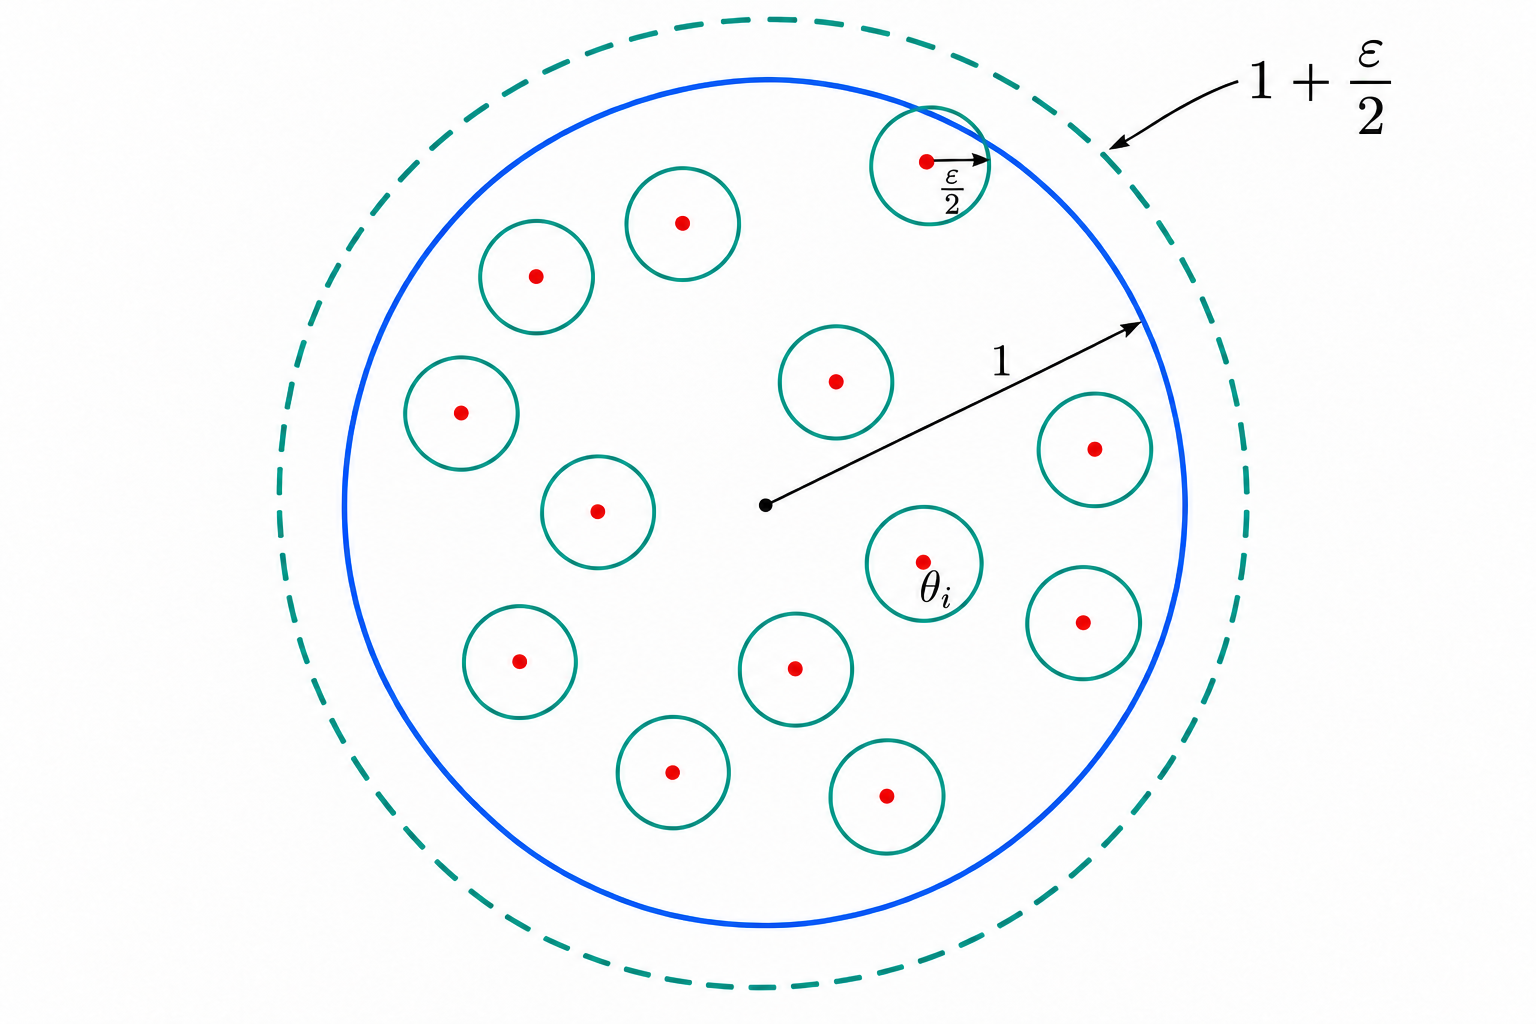
\includegraphics[width=0.76\textwidth]{./lec6-covering-volume.png}

  \small Volume comparison for an $\epsilon$-packing. The blue circle is the unit ball; the dashed circle has radius $1+\epsilon/2$. Each small ball has radius $\epsilon/2$ and is centered at a packing point. Schematic, not to scale.
\end{center}
This implies that
\begin{align*}
  M \cdot \vol(\ball_2^d (\epsilon/2)) \leq \vol(\ball_2^d (1 + \epsilon/2)),
\end{align*}
which gives us
\begin{align*}
  M \leq \Big( 1 + \frac{2}{\epsilon} \Big)^d,
\end{align*}
and by duality, we have
\begin{align*}
  N (K; \|\cdot\|_2, \epsilon) \leq \Big( 1 + \frac{2}{\epsilon} \Big)^d.
\end{align*}

\paragraph{Lower bound:} Suppose $(\psi_i)_{i = 1}^N$ is an $\epsilon$-covering of $K$. Then we have
\begin{align*}
  \vol (\ball_2^d (1)) \leq N \cdot \vol(\ball_2^d (\epsilon)),
\end{align*}
which gives us
\begin{align*}
  N \geq \frac{\vol (\ball_2^d (1))}{\vol(\ball_2^d (\epsilon))} = \Big( \frac{1}{\epsilon} \Big)^d.
\end{align*}
Technically, the gap between the upper bound and lower bound is a factor of $2^d$. But in statistical applications, we usually use log covering number, and the resulting difference is just a constant factor. In particular, we have
\begin{align*}
  \log N (K; \|\cdot\|_2, \epsilon) \asymp d \log (1/\epsilon).
\end{align*}
\section{Application to $M$-estimation}
Recall that we are interested in
\begin{align*}
  \thetahat_n \in \arg\min_{\theta \in \Theta} F_n (\theta), \quad \theta^* \in \arg\min_{\theta \in \Theta} F (\theta).
\end{align*}
We need to show uniform convergence of $F_n (\theta)$ to $F (\theta)$.
\begin{theorem}[Wald]
  Suppose that $\Theta$ is compact (with respect to some metric $\rho$), and $f (x; \theta)$ is continuous in $\theta$ (with respect to $\rho$) for each $x$. Suppose furthermore that
  \begin{align*}
    \Exs \Big[ \sup_{\theta \in \Theta} f (X; \theta) \Big] < + \infty.
  \end{align*}
  (i.e., the class has an integrable envelope function). Then we have
  \begin{align*}
    \sup_{\theta \in \Theta} |F_n (\theta) - F (\theta)| \xrightarrow{p} 0.
  \end{align*}
\end{theorem}

\paragraph{Proof.} Fix $\varepsilon > 0$. Since $f (x; \theta)$ is continuous in $\theta$ and $\Theta$ is compact, we know that $F$ is uniformly continuous on $\Theta$. Therefore, there exists $\delta > 0$ such that for any $\theta_1, \theta_2 \in \Theta$ with $\rho(\theta_1, \theta_2) < \delta$, we have $|F (\theta_1) - F (\theta_2)| < \varepsilon$. (This is used to control the discretization error).

Let $(\theta_i)_{i = 1}^N$ be a $\delta$-covering of $\Theta$. Since the set $\Theta$ is compact, we know that $N < +\infty$.
\begin{align*}
  \sup_{\theta \in \Theta} |F_n (\theta) - F (\theta)| &\leq \max_{i = 1, \cdots, N} \sup_{\theta: \rho (\theta, \theta_i) \leq \delta} \Big\{\underbrace{|F_n (\theta_i) - F (\theta_i)|}_{\max_{i} (\cdots) \xrightarrow{p} 0, ~{\color{red} T_1}} + \underbrace{|F (\theta_i) - F (\theta)|}_{\leq \varepsilon} + \underbrace{|F_n (\theta) - F_n (\theta_i)|}_{\text{problematic term},~ {\color{red} T_3}} \Big\}
\end{align*}
We can upper bound the problematic term as follows:
\begin{align*}
  \mathrm{problematic term} &=  \max_{i = 1, \cdots, N} \sup_{\theta: \rho (\theta, \theta_i) \leq \delta} \Big| \frac{1}{n} \sum_{j=1}^n \big( f (X_j; \theta) - f (X_j; \theta_i) \big) \Big |\\
  &\leq \max_{i = 1, \cdots, N}  \frac{1}{n} \sum_{j=1}^n  \underbrace{\sup_{\theta: \rho (\theta, \theta_i) \leq \delta} \big| f (X_j; \theta) - f (X_j; \theta_i) \big|}_{\text{i.i.d. average of this}}
\end{align*}
By law of large numbers, we have
\begin{align*}
  \max_{i = 1, \cdots, N}  \frac{1}{n} \sum_{j=1}^n  \sup_{\theta: \rho (\theta, \theta_i) \leq \delta} \big| f (X_j; \theta) - f (X_j; \theta_i) \big| &\xrightarrow{p} \max_{i = 1, \cdots, N} \Exs \Big[ \sup_{\theta: \rho (\theta, \theta_i) \leq \delta} \big| f (X; \theta) - f (X; \theta_i) \big| \Big]\\
  &\leq \sup_{\theta \in K} \Exs \Big[ \sup_{\theta': \rho (\theta, \theta') \leq \delta} \big| f (X; \theta) - f (X; \theta') \big| \Big],
\end{align*}
which is the worst-case modulus-of-continuity of $f (X; \theta)$ in $\theta$, at scale $\delta$.

For any $\theta \in \Theta$, define
\begin{align*}
  M_\delta (\theta) \mydefn \sup_{\theta': \rho (\theta, \theta') \leq \delta} \big| f (X; \theta) - f (X; \theta') \big|.
\end{align*}
We know that for each fixed $\theta$, we have pointwise convergence $M_\delta (\theta) \to 0$ as $\delta \to 0$, by continuity of $f (X; \theta)$ in $\theta$. On the other hand, we also have $M_\delta (\theta) \leq 2 \sup_{\theta \in \Theta} |f (X; \theta)|$, which is integrable by assumption. Therefore, by dominated convergence theorem, we have
\begin{align*}
  \Exs [M_\delta (\theta)] \rightarrow 0, \qquad \forall \theta \in \Theta.
\end{align*}
By Dini's theorem and the compactness of $\Theta$, we know that the convergence is uniform in $\theta$.

\paragraph{Remarks:}
\begin{enumerate}
  \item This only needs very weak conditions, but only proves asymptotic convergence.
  \item Using this result, and in combination with basic inequality, we have $F(\thetahat_n) - F (\theta^*) \xrightarrow{p} 0$. Furthermore, under the same setup, $F$ is continuous, and assuming that $\theta^*$ is unique minimizer, then we have $\thetahat_n \xrightarrow{p} \theta^*$.
  \item Can we turn this into a more quantitative bound?
\end{enumerate}
For the term $\color{red} T_1$, we note that
\begin{align*}
  &\Prob \Big( \max_{i = 1, \cdots, N} |F_n (\theta_i) - F (\theta_i)| > \varepsilon \Big)\\
  &\qquad\leq \sum_{i = 1}^N \Prob (|F_n (\theta_i) - F (\theta_i)| > \varepsilon)\\
  &\qquad\leq N \cdot \max_{i = 1, \cdots, N} \Prob (|F_n (\theta_i) - F (\theta_i)| > \varepsilon).
\end{align*}
If $f$ is bounded by $1$, then we can use Hoeffding's inequality to get
\begin{align*}
  \Prob \Big( \max_{i = 1, \cdots, N} |F_n (\theta_i) - F (\theta_i)| > \varepsilon \Big) \leq 2N e^{-2n\varepsilon^2}.
\end{align*}
By taking $\varepsilon = \sqrt{\frac{\log (2N / \delta)}{2n}}$,  we have the high-probability bound.

On the other hand, if $f$ is unbounded (or even heavy-tailed), we cannot directly apply Hoeffding's inequality. Na\"{i}ve application of Chebyshev's inequality gives us $\varepsilon \asymp \sqrt{N / n}$, which is not useful when $N$ is large.

This can be overcome by ``symmetrization method'' and Rademacher complexity.

\bigskip
For the term $\color{red} T_3$, we can bound it as long as we have quantitative bound on the modulus-of-continuity of $f (X; \theta)$ in $\theta$. But on the other hand, this type of one-step discretization argument is fundamentally sub-optimal. We can do better by using ``chaining method'', which is a multi-step discretization argument.

\section{Symmetrization and chaining methods}

\subsection{Symmetrization method}
Introducing the notations:
\begin{align*}
  P_n f = \frac{1}{n} \sum_{i = 1}^n f (X_i), \quad P f = \Exs [f (X)], \quad (P_n - P) f = P_n f - P f.
\end{align*}
For notation simplicity, we drop the parametrization by $\theta$ and write $f (X)$ instead of $f (X; \theta)$. We are interested in bounding
\begin{align*}
  \Exs \Big[\sup_{f \in \mathcal{F}} |(P_n - P) f| \Big].
\end{align*}
Here $\mathcal{F} = \{f (X; \theta): \theta \in \Theta\}$ is the function class induced by the parametrization $\theta \in \Theta$.

The ``symmetrized version'' of the above quantity is
\begin{align*}
  \mathcal{R}_n (\mathcal{F}) \mydefn \Exs \Big[ \sup_{f \in \mathcal{F}} \Big| \frac{1}{n} \sum_{i = 1}^n \varepsilon_i f (X_i) \Big| \Big], \quad \varepsilon_i \simiid \mathrm{Rademacher} (\pm 1),
\end{align*}
which is called the Rademacher complexity of the function class $\mathcal{F}$. The Rademacher complexity is a measure of the richness of the function class $\mathcal{F}$, and it is often easier to bound than the original quantity, because we can bound it by conditioning on $X_1, \cdots, X_n$ and using concentration inequalities for Rademacher random variables.

\begin{theorem}[symmetrization]
  We have
  \begin{align*}
    \Exs \Big[\sup_{f \in \mathcal{F}} |(P_n - P) f| \Big] \leq 2 \mathcal{R}_n (\mathcal{F}).
  \end{align*}
\end{theorem}
Proof: Let $X_1', \cdots, X_n' \simiid \Prob$ be an independent copy of $X_1, \cdots, X_n$. Then we have
\begin{align*}
\Exs \Big[ \sup_{f \in \mathcal{F}} |(P_n - P)f| \Big] &= \Exs \Big[ \sup_{f \in \mathcal{F}} \Big| \frac{1}{n} \sum_{i = 1}^n \big(f (X_i) - \Exs [f (X_i')] \big) \Big| \Big]\\
&\overset{(\text{Jensen})}{\leq} \Exs \Big[ \sup_{f \in \mathcal{F}} \Big| \frac{1}{n} \sum_{i = 1}^n \big(f (X_i) - f (X_i') \big) \Big| \Big]
\end{align*}
We know that by introducing Rademacher random variables $\varepsilon_i \simiid \mathrm{Rademacher} (\pm 1)$, we have
\begin{align*}
  \big( f(X_i) - f (X_i') \big)_{i = 1}^n \overset{d}{=} \big( \varepsilon_i (f(X_i) - f (X_i')) \big)_{i = 1}^n,
\end{align*}
so we have
\begin{align*}
  \text{above} &= \Exs \Big[ \sup_{f \in \mathcal{F}} \Big| \frac{1}{n} \sum_{i = 1}^n \varepsilon_i (f(X_i) - f (X_i')) \Big| \Big] \leq 2 \mathcal{R}_n (\mathcal{F}).
\end{align*}

\paragraph{Application of symmetrization method:} We can reason conditionally on $X_1, \cdots, X_n$, and Rademacher random variables are bounded and nicely behaved in terms of concentration inequalities.

In particular, for any $A \subseteq \real^n$, we define the Rademacher complexity of $A$ as
\begin{align*}
  R_n (A) \mydefn \Exs \Big[ \sup_{a \in A} \Big| \frac{1}{n} \sum_{i = 1}^n \varepsilon_i a_i \Big| \Big], \quad \varepsilon_i \simiid \mathrm{Rademacher} (\pm 1).
\end{align*}
This has nothing to do with the data or statistical problem, and is purely a combinatorial measure of the complexity of the set $A$.

Following the arguments in the previous section, we can bound it using concentration inequality.

\paragraph{For finite $A$:} for any $\lambda > 0$, by Jensen's inequality,
\begin{align*}
  R_n (A) &\leq \frac{1}{\lambda} \log \Exs \Big[ \max_{a \in A \cup (- A)} \exp \Big( \lambda  \frac{1}{n} \sum_{i = 1}^n \varepsilon_i a_i  \Big) \Big]\\
  &\leq \frac{1}{\lambda}  \log \Big\{ \sum_{a \in A \cup (-A)} \Exs \Big[  \exp \Big( \lambda  \frac{1}{n} \sum_{i = 1}^n \varepsilon_i a_i  \Big) \Big] \Big\}\\
  &\leq \frac{\log (2 |A|)}{\lambda} + \frac{\lambda}{2 n^2} \max_{a \in A} \sum_{i = 1}^n a_i^2\\
  &\overset{\text{(choosing optimal $\lambda$)}}{=} \sqrt{\frac{2 \log (2 |A|)}{n}} \cdot \max_{a \in A} \sqrt{\frac{\sum_{i = 1}^n a_i^2}{n}}.
\end{align*}

\subsection{Discretization and chaining}
Following the same idea as before, we bound $R_n (A)$ for an infinite set $A \subseteq \real^n$.

\paragraph{One-step discretization:}
Let $(a^{(i)})_{i = 1}^N$ be an $\varepsilon$-covering of $A$ with respect to the normalized metric
\begin{align*}
  \vecnorm{a}{n} = \sqrt{\frac{1}{n} \sum_{i = 1}^n a_i^2}.
\end{align*}
Denote $\pi (a) \mydefn \arg\min_{a^{(i)}} \vecnorm{a - a^{(i)}}{n}$ as the projection of $a$ onto the covering set. Then we have
\begin{align*}
R_n(A) &\leq \underbrace{\Exs \Big[ \sup_{a \in A} n^{-1}|\varepsilon^\top (a - \pi(a))| \Big]}_{(\text{C.--S.})\quad \leq \sup_{a \in A} \vecnorm{a - \pi (a)}{n}} + \underbrace{\Exs \Big[ \sup_{a \in A} n^{-1}|\varepsilon^\top \pi(a)| \Big] }_{\leq \sqrt{\frac{2\log (2 N)}{n}} \cdot \mathrm{diam} (A)}\\
&\leq \varepsilon + \sqrt{\frac{2\log (2 N (\varepsilon))}{n}} \cdot \mathrm{diam} (A).
\end{align*}
Is this argument tight?

Consider $A$ being a unit ball in $d$-dimensional subspace (this could come from using a $d$-dimensional linear model for $\mathcal{F}$) By choosing $\varepsilon = O (1/n)$, we have
\begin{align*}
  R_n (A) \leq O (\sqrt{\frac{d \log n }{ n}}).
\end{align*}
For linear model, by doing direct calculation, we can show that $R_n (A) \asymp \sqrt{d / n}$. So the above bound is sub-optimal by a factor of $\sqrt{\log n}$. In general, this sub-optimality can go beyond log factors for nonparametric function classes.

\paragraph{Multi-step discretization:} Potential looseness of one-step discretization: $(a - \pi (a))$ may contain some structures, but we just bound it using Cauchy--Schwarz.

Now let us consider a sequence of discrete approximations to $A$ (not necessarily nested).
\begin{align*}
  \{0\} = A_0, A_1, \cdots, A_m, \cdots
\end{align*}
Denote $\pi_m (a) \mydefn \arg\min_{a^{(i)} \in A_m} \vecnorm{a - a^{(i)}}{n}$ as the projection of $a$ onto the $m$-th covering set.

Concretely, we choose $A_m$ to be $\delta_m$-covering of $A$ with respect to the normalized metric $\vecnorm{\cdot}{n}$ (with $\delta_m \downarrow 0$ to be chosen). For each $a \in A$, we have the decomposition
\begin{align*}
  a = \sum_{m = 0}^\infty \big( \pi_{m + 1} (a) - \pi_{m } (a) \big).
\end{align*}
So we have
\begin{align*}
  \Exs \Big[ \sup_{a \in A} n^{-1} |\varepsilon^\top a| \Big] \leq \sum_{m = 0}^\infty \Exs \Big[ \sup_{a \in A} n^{-1} |\varepsilon^\top (\pi_{m + 1} (a) - \pi_m (a))| \Big].
\end{align*}
Each term measures the complexity at scale $\delta_m$, and each term takes supremum over a finite set. So we have
\begin{align*}
  \Exs \Big[ \sup_{a \in A} n^{-1} |\varepsilon^\top (\pi_{m + 1} (a) - \pi_m (a))| \Big] \leq (\delta_m + \delta_{m + 1}) \cdot \sqrt{\frac{2 \log |A_m| \cdot |A_{m + 1}|}{n}}
\end{align*}

By manipulating this type of bounds carefully, we can arrive at a nice form
\begin{theorem}[Dudley's chaining bound]
  There exists a universal constant $c > 0$ such that
  \begin{align*}
    R_n (A) \leq c\int_0^{\mathrm{diam} (A)} \sqrt{\frac{\log N (A; \vecnorm{\cdot}{n}, \epsilon)}{n}} d \epsilon.
  \end{align*}
\end{theorem}
Proof: Let $D$ be the diameter of $A$ under $\vecnorm{\cdot}{n}$. Let $\delta_m = 2^{-m} D$, and we have
\begin{align*}
\delta_m + \delta_{m + 1} = 3 \cdot 2^{-m - 1} D, \quad  |A_m| \cdot |A_{m + 1}| \leq |A_{m + 1}|^2 = N (A; \vecnorm{\cdot}{n}, \delta_{m + 1})^2.
\end{align*}
Substituting to the bound, we have
\begin{align*}
  R_n (A) \leq \sum_{m = 0}^\infty 3 \cdot 2^{-m - 1} D \cdot \sqrt{\frac{4 \log N (A; \vecnorm{\cdot}{n}, \delta_{m + 1})}{n}}
\end{align*}
To compare this dyadic sum with an integral, put
\begin{align*}
  g(\epsilon) = \sqrt{\frac{\log N(A;\vecnorm{\cdot}{n},\epsilon)}{n}}.
\end{align*}
The covering number, and hence $g$, is nonincreasing in $\epsilon$.
On $[\delta_{m+2},\delta_{m+1}]$, we therefore have
$g(\epsilon)\geq g(\delta_{m+1})$. Since
$\delta_{m+2}=\delta_{m+1}/2$, the rectangle shown below gives
\begin{align}
  \delta_{m+1}g(\delta_{m+1})
  \leq 2\int_{\delta_{m+2}}^{\delta_{m+1}}g(\epsilon)\,d\epsilon.
  \label{eq:lec6-dyadic-rectangle}
\end{align}
\begin{center}
  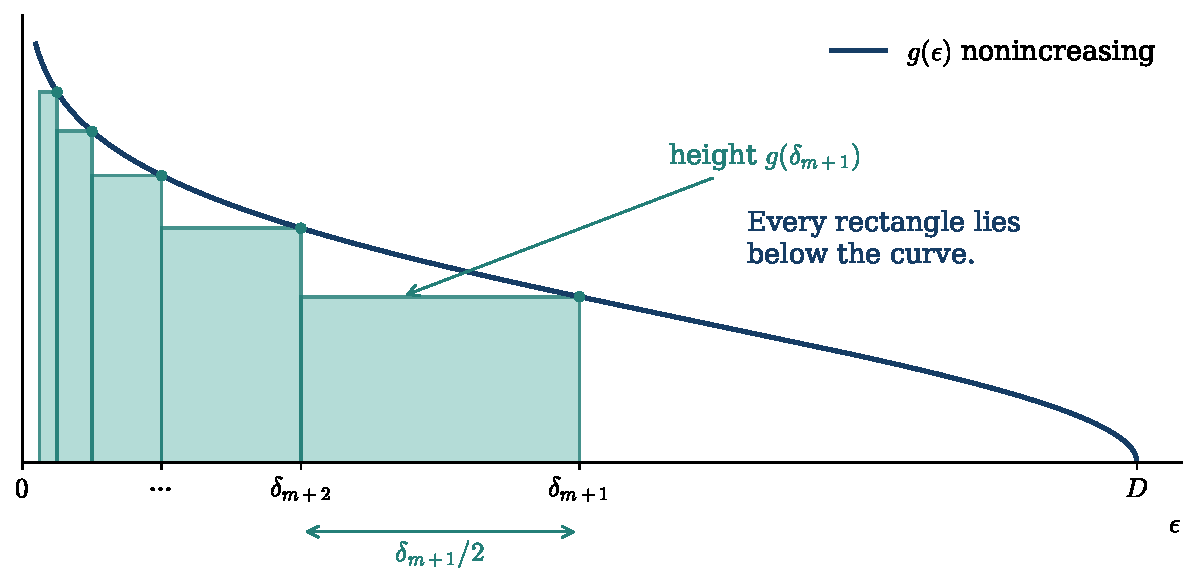
\includegraphics[width=0.9\textwidth]{./lec6-dyadic-integral.pdf}

  \small Right-endpoint rectangles lie below a nonincreasing curve. The displayed curve is illustrative; the same area comparison applies to the entropy function $g$ above.
\end{center}
The preceding chaining sum is $6\sum_{m\geq0}\delta_{m+1}g(\delta_{m+1})$.
Summing~\eqref{eq:lec6-dyadic-rectangle} over disjoint adjacent intervals yields
\begin{align*}
  6\sum_{m=0}^{\infty}\delta_{m+1}g(\delta_{m+1})
  &\leq 12\int_0^{D/2}g(\epsilon)\,d\epsilon\\
  &\leq 12\int_0^D g(\epsilon)\,d\epsilon.
\end{align*}
This proves the sum-to-integral comparison, including the constant factor.
For an infinite sum, apply the comparison first to finite partial sums and then use monotone convergence; if the integral diverges, the inequality remains valid but is uninformative.

\bigskip
\noindent \textbf{Remarks}:
\begin{itemize}
  \item Dudley integral may diverge in certain case (when the log-covering number grows too fast). In this case, you may consider a truncated version of the integral. Using a finite collection of scales, and bounding the rest using Cauchy--Schwarz, we can still get a finite bound.
  \begin{align*}
    R_n (A) \leq \delta + c\int_\delta^{\mathrm{diam} (A)} \sqrt{\frac{\log N (A; \vecnorm{\cdot}{n}, \epsilon)}{n}} d \epsilon.
  \end{align*}
  You can further optimize over $\delta$ to get the best bound.
  \item Dudley's chaining bound is tight for many function classes, but not always. There are more advanced chaining techniques (generic chaining) that can give tight bounds for all function classes.
\end{itemize}

\subsection{Back to function classes}
Recall that we want to bound $\Exs \Big[\sup_{f \in \mathcal{F}} |(P_n - P) f| \Big]$. We assume (as in Wald's theorem) that $\mathcal{F}$ has an envelope function $G$, i.e., $|f (X)| \leq G (X)$ for all $f \in \mathcal{F}$. But here we assume that $\Exs [G^2 (X)] < + \infty$.

\begin{theorem}
  Under above setup, we have
  \begin{align*}
    \Exs \Big[\sup_{f \in \mathcal{F}} |(P_n - P) f| \Big] \leq c \sqrt{\frac{\Exs [G^2 (X)]}{n}}\int_0^{1} \sqrt{\log \sup_{Q} N (\mathcal{F}; \mathbb{L}^2 (Q), \vecnorm{G}{\mathbb{L}^2 (Q)} \epsilon)} d \epsilon,
  \end{align*}
\end{theorem}
Chaining under the worst-case distribution $Q$.

Proof: Using symmetrization and chaining, we have the conditional expectation bound:
\begin{align*}
  \Exs \Big[ \sup_{f \in \mathcal{F}} |(P_n - P) f|  \Big| X_1, \ldots, X_n \Big] \leq \frac{c}{\sqrt{n}} \int_0^{\sqrt{P_n G^2}} \sqrt{\log N (\mathcal{F}; \mathbb{L}^2 (P_n), \epsilon)} d \epsilon.
\end{align*}
The metric and integral upper limit are data-dependent. We use change-of-variable to pull this integral upper limit outside, and then replace $P_n$ using the worst-case distribution $Q$ to get the final bound. For the envelope function, we use the bound
\begin{align*}
  \Exs \big[ \sqrt{P_n G^2} \big] \leq \sqrt{\Exs [P_n G^2]} = \sqrt{\Exs [G^2 (X)]}.
\end{align*}

\end{document}
